% 2500 words

\section{RQ1: Predicting attractiveness from spatial features}
\subsubsection*{Prediction model evaluation and selection}

As previously explained, choosing a suitable machine learning model is critical, as Machine Learning explanation techniques such as SHAP would be less insightful if the predictions produced high inaccuracies. The evaluation results in Table \ref{tab:modeleval} show that the Gradient Boosting tree-based model (XGBoost) outperforms the other models in predicting the target variable \textit{Total arrivals (log)} with an $R^2$ of 0.792. Meanwhile, the simple Linear Regression model performs more poorly in comparison due to underfitting (i.e., consistently low accuracy with training data folds), and the Multilayer Perceptron Artificial Neural Network model also performs poorly but due to overfitting (i.e., high accuracy achieved with training data folds but low accuracy with validation data folds). XGBoost also outperforms itself when predicting the pre-transformed target variable with an $R^2$ of 0.633. This shows that while XGBoost has long been popular thanks to its fast convergence and high validation accuracy, transforming the highly right-skewed target variable can further improve prediction performance. 

\begin{table}[ht]
    \centering
    \renewcommand{\arraystretch}{1.5}
    \begin{tabular}{|c|c|c|}
        \hline
        \rowcolor{lightgray}
        \textbf{Model} & \textbf{$R^2$ (raw)} & \textbf{$R^2$ (log)} \\
        \hline
        Linear Regression & 0.576 & 0.697 \\
        \rowcolor{pink}
        XGBoost & 0.633 & \textbf{0.792} \\
        ANN & 0.526 & 0.410\\
        \hline
    \end{tabular}
    \captionsetup{justification=centering}
    \caption{Comparing model $R^2$ results of 3 models predicting \\Total arrivals (raw) and Total arrivals (log) \\using spatial k-fold cross-validation for tuning and evaluation}
    \label{tab:modeleval}
\end{table}

\begin{table}[ht]
    \centering
    \renewcommand{\arraystretch}{1.5}
    \begin{tabular}{|c|c|c|c|}
        \hline
        \rowcolor{lightgray}
        \textbf{Timeband} & \textbf{R$^2$} & \textbf{MSE} & \textbf{MAE} \\
        \hline
        Total   & \textbf{0.823} & 0.687 & 0.570 \\
        Morning & \textbf{0.809} & 0.614 & 0.571 \\
        Midday  & \textbf{0.828} & 0.629 & 0.549 \\
        Evening & \textbf{0.819} & 0.687 & 0.593 \\
        Late    & \textbf{0.824} & 0.635 & 0.601 \\
        \hline
    \end{tabular}
    \captionsetup{justification=centering}
    \caption{Finetuned XGBoost model evaluation results for All target variables (log)\\using nested spatial k-fold cross-validation for tuning and evaluation}
    \label{tab:modelevaltimeband}
\end{table}

\begin{figure}[!hbt]
    \centering
    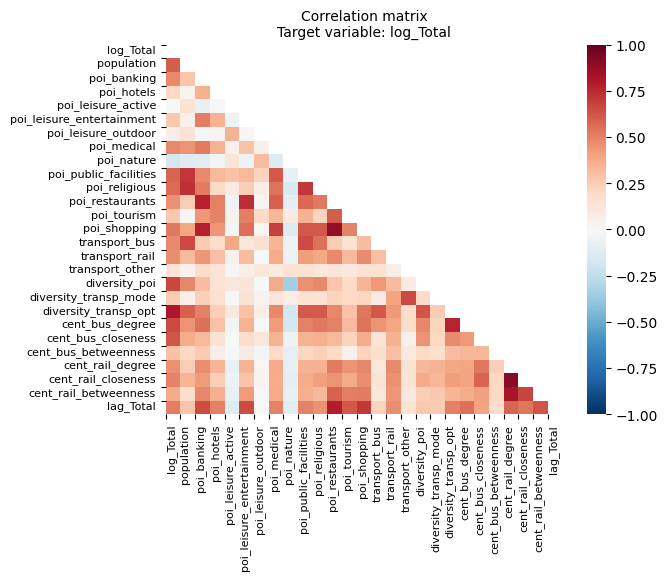
\includegraphics[width=0.8\textwidth]{correlation.png}
    \captionsetup{justification=centering}
    \caption{Correlation matrix of the input features and target variable Total arrivals (log)}
    \label{fig:corrmatt}
\end{figure}

In managing overfitting risks, XGBoost stands out among other models for its built-in L1 and L2 regularisation hyperparameters, which penalise the model for complexity and suppress highly correlated input features. This is particularly important when considering the complex patterns of correlations among our input features, as shown in Figure \ref{fig:corrmatt}. Here we observe groups of highly correlated features, such as Population-Public Facilities-Religious POIs, Entertainment-Restautants-Shopping POIs, and between different public transport centrality measures. Therefore, with XGBoost, we could further fine-tune two hyperparameters \textit{alpha} and \textit{lambda}---which represent L1 and L2 regularisation thresholds, respectively---to achieve even better prediction results. As done previously, nested spatial k-fold cross-validation is used to fine-tune the model and validate the results. The fine-tuned XGBoost model improves $R^2$ up to \textbf{0.823} (an approx. 3pp increase) in predicting total arrivals from the pre-tuned model and performs consistently well in predicting arrivals by time band, as shown in Table \ref{tab:modelevaltimeband}. The results suggest that the fine-tuned XGBoost model is fit for purpose and enables us to address the first research question: Built environment features engineered from open data are adequate predictors of public transport inflows (as a proxy for trip attractiveness) to a high degree of accuracy.

Before further analysis, it is important to recognise where the model falls short and what that may tell us about its potential lack of generalisability. Figure \ref{fig:outliers} shows the distribution of observations whose prediction residuals are Tukey's fence's 'outliers', i.e., the target variables are significantly overpredicted or underpredicted. These are primarily concentrated in Outer London where poor predictions go in both directions. While it is not easy to immediately unravel, possible root causes include: 

\begin{itemize}
    \setlength\itemsep{0em}
    \item \textit{Low Spatial Autocorrelation:} There is consistency between areas with low spatial autocorrelation of the target variable (see Figure \ref{fig:lisacluster}, grey regions), and where the model predicts more poorly. This may indicate that incorporating spatial lag as a feature improves the model's performance only where spatial autocorrelation is present. In its absence, the model has a higher chance of poorer predictions based on the main features alone.
    \item \textit{Omitted features:} It is possible that adding variables such as car ownership and socioeconomic factors can help the model predict two hypothetical areas with the same built environment profiles but different public transport usage. This is especially true in Outer London, where car ownership is higher, and public transport services are less frequent.
    \item \textit{Incomplete target variable:} It is probable that a spatial unit with its built environment profile does have the predicted public transport trip attractiveness in reality. However, since only data from TfL-operated services are considered, omitting trip data from other rail operators---more prevalent in Outer London and especially south of the Thames--- may manifest as an apparent overprediction. 
\end{itemize}

\begin{figure}[hbt]
    \centering
    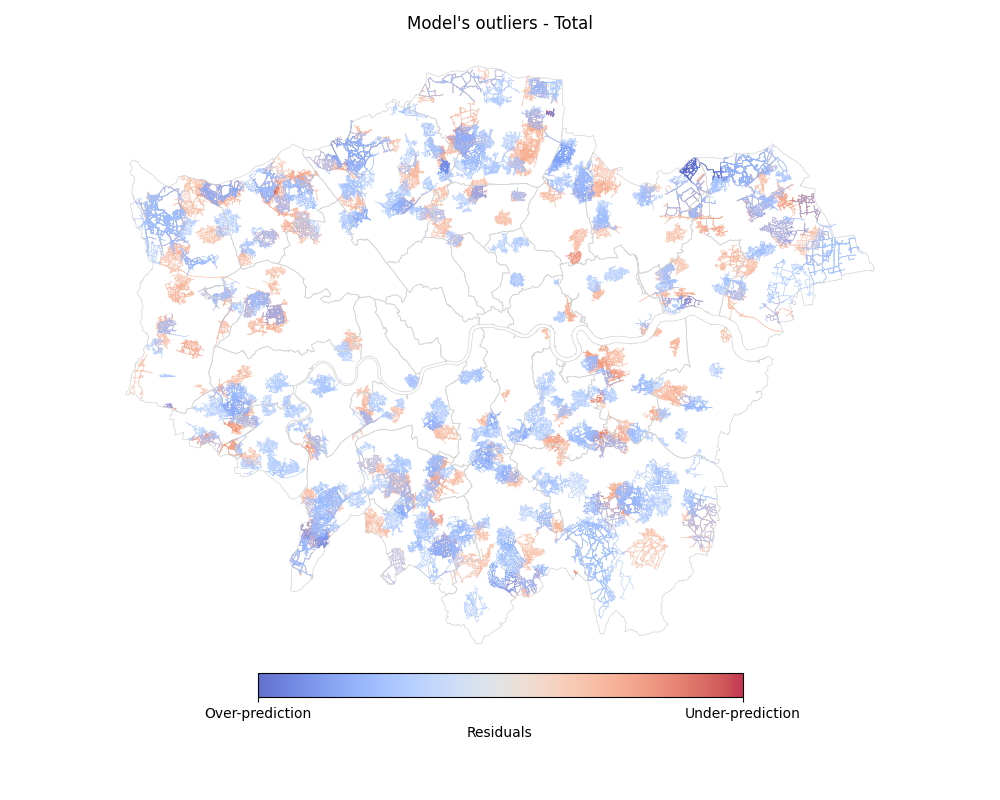
\includegraphics[width=0.6\textwidth]{outliers.png}
    \captionsetup{justification=centering}
    \caption{Observations with significant overprediction and underprediction (N=576 of 16,890)\\Fine-tuned XGBoost model, Total arrivals (log)}
    \label{fig:outliers}
\end{figure}

Nonetheless, these 'outliers' account for less than 3.5\% of the total observations, and the model's performance is still satisfactory in explaining the large majority of the spatial units in the Greater London area. 

\subsubsection*{Global feature importance}

After fitting the fine-tuned XGBoost model to the entire dataset, we applied SHAP to obtain the SHAP values for each feature and observation. This allows us to evaluate the importance of each feature in predicting the target variable and understand the direction of the relationship between the feature and the target variable. 

Figure \ref{fig:beeswarmtotal} shows the summary of feature importance for the target variable \textit{Total arrivals (log)} from most to least important (top to bottom) as distributions of the SHAP values for each feature. For each feature, the direction of the relationship between the feature value and the SHAP values is shown using a red-blue scale: For example, the higher the value of the feature \textit{Rail transport node density (transport\_rail)}, the likelier it contributes positively to the prediction (red tail on the right side). Meanwhile, the higher the value of the feature \textit{Leisure-Active POI density (poi\_leisure\_active)}, the likelier it contributes negatively to the prediction (red tail on the left side). For the feature \textit{Closeness centrality measure on the bus network (cent\_bus\_closeness)}, higher feature values have a weaker positive impact on the prediction, while lower feature values have a stronger negative impact on the prediction (i.e., the distribution has a longer blue tail on the left side than the red tail on the right side).

From here, we can make several observations: First, the connectivity profile features have outsized importance with the \textit{transport route option diversity index (diversity\_transp\_opt)} on top in predicting trip attractiveness. This is consistent with the reality that people tend to alight/exit at transport-rich areas with multiple bus routes or rail services for onward journeys, representing the most prominent interchange behaviour. The second most important feature is the spatial lag of the target variable (i.e., mean of target variables of neighbouring), which partially corroborates its influence on the model's performance hypothesised earlier when analysing outliers. The most important amenity POI feature is \textit{shopping POIs}, which is also consistent impact across all time bands (see Figure \ref{fig:beeswarmtimeband} in Appendix), followed by \textit{banking POIs}, \textit{active leisure POIs}, \textit{medical POIs}, \textit{restaurant POIs}, \textit{nature POIs}, and \textit{outdoor leisure POIs}. This suggests that for the whole of Greater London, total arrivals as a proxy for trip attractiveness are driven mainly by, first and foremost, the need to interchange for onward travel and, secondly, by the availability of certain key types of amenities.

\begin{figure}[!hbt]
    \centering
    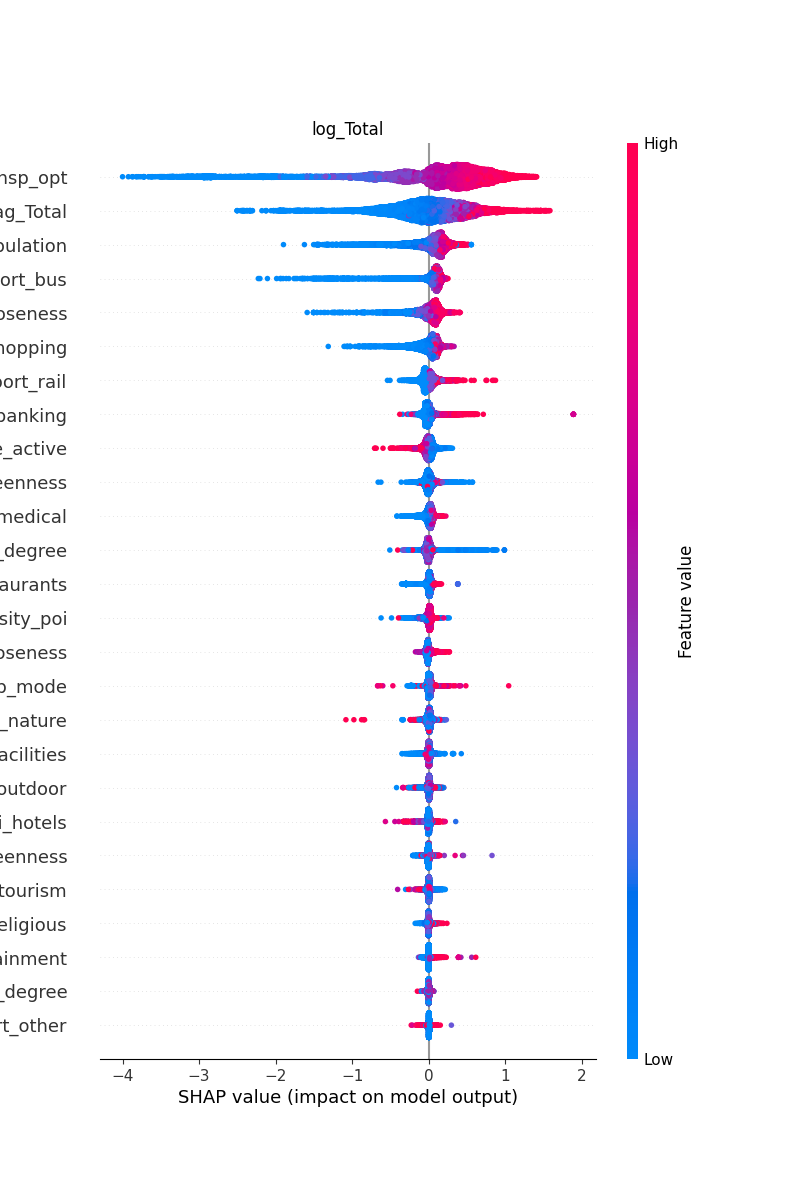
\includegraphics[width=0.5\textwidth]{beeswarm_log_Total.png}
    \captionsetup{justification=centering}
    \caption{Summary of feature importance based on SHAP values. Red-Blue scale represents the feature value, and the x-axis represents the SHAP value, i.e., impact on final model prediction of Total arrivals (log)}
    \label{fig:beeswarmtotal}
\end{figure}

At this point, it is important to acknowledge the effect of correlation between the input features as previously observed and how the XGBoost model learns on SHAP global explanations. Although XGBoost's regularisation hyperparameters are in place to avoid overfitting due to highly correlated features, they do not drop them from the model. Consequently, when SHAP is applied for a retroactive explanation, highly correlated features will show comparable importance. Therefore, it is more insightful to consider the SHAP values of the correlated features in clusters, as shown in Figure \ref{fig:barclustertotal}. We can see that there are differences from the previous graph, where the top most important features (or feature clusters) are as follows:

\begin{enumerate}
    \setlength\itemsep{-0.3em}
    \item Transport route option diversity index
    \item Spatial Lag
    \item Population + Public Facilities (clustered, local residential amenity features)
    \item Bus stop density + Bus stop closeness centrality (clustered, bus interchange features)
    \item Shopping and Restaurants POI density (clustered, commercial features)
\end{enumerate}

\begin{figure}[ht]
    \centering
    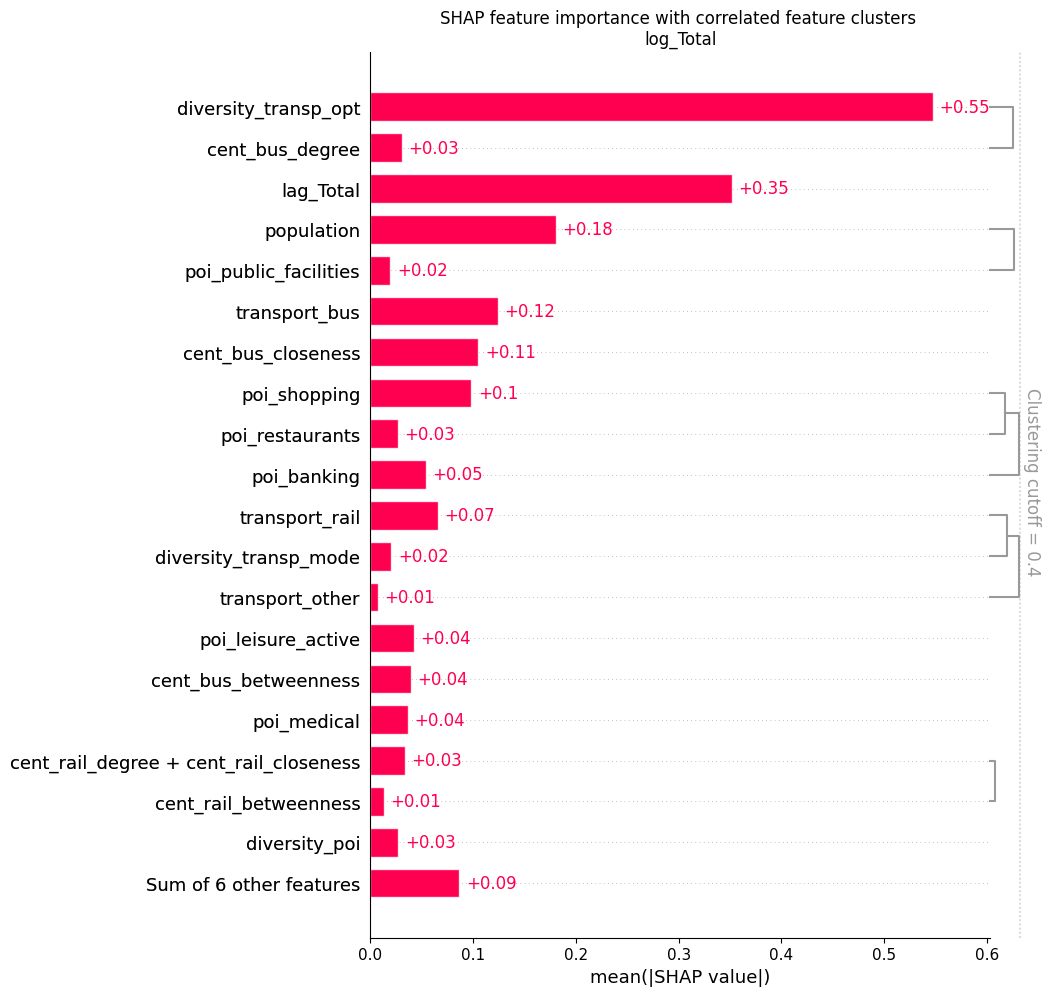
\includegraphics[width=0.5\textwidth]{new_barclus_log_Total.png}
    \captionsetup{justification=centering}
    \caption{Feature importance in predicting Total arrivals (log)\\ Features clustered by correlation and ordered by mean absolute SHAP values}
    \label{fig:barclustertotal}
\end{figure}

In summary, as it pertains to our first research question, the global feature importance analysis shows that built environment features are indeed important predictors of public transport inflow demand in London and that the XGBoost model can capture the complex relationships between these features and the target variable with high accuracy ($>80\%$). There are also opportunities to improve the prediction performance by addressing possibly omitted spatial and non-spatial features. The high importance of the spatial lag feature is both an advantage and a shortcoming: While it drastically improves the model's performance overall for Greater London, it penalises the model in areas where the spatial autocorrelation is low, reducing its generalisability to predicting the trip attractiveness of an isolated area without considering its neighbours. Finally, highly correlated features should be considered in clusters when analysing importance to avoid interpreting undue importance to a single feature.

\pagebreak[4]
\section{RQ2: Identifying local attractors and hotspots}

One of the highlights of SHAP is its ability to provide local explanations for individual predictions. When applied to a spatial system, these local explanations offer additional insights on spatial phenomena that are not well captured in a global feature importance analysis, namely spatial heterogeneity (i.e., varying impact of the target variable across different spatial units) and spatial non-stationarity (i.e., varying impact of an input feature on the target variable across different spatial units). SHAP's additive property allows us to decompose the prediction of a spatial unit into the sum of the SHAP values of each feature and exact the contribution of each feature to the prediction.

Figure \ref{fig:localshap} shows the local SHAP values for two spatial units, Kew Gardens and Covent Garden, for a closer look. They represent two distinct localities with supposedly different amenity and transport profiles. Kew Gardens is a quiet residential area in the public transport network, also known for its many renowned parks and gardens, while Covent Garden is a bustling commercial and entertainment district with high connectivity in the public transport network. The local SHAP values for Kew Gardens show a higher contribution of the population density and POI classes associated with neighbourhood amenities (stores, clinics, etc.) to the prediction of total arrivals. In comparison, the local SHAP values for Covent Garden show a higher contribution of POI classes such as restaurants, entertainment venues, etc. This is consistent with the expected profiles of the two areas and demonstrates SHAP's ability to provide local explanations for individual predictions. In both cases, in line with global feature importance, the transport route option index's contribution is among the top, indicating that with the station exit and bus alighting dataset at hand, the interchange behaviour is still a significant pattern regardless of where in London the spatial unit is located.

\begin{figure}[!ht]
    \centering
    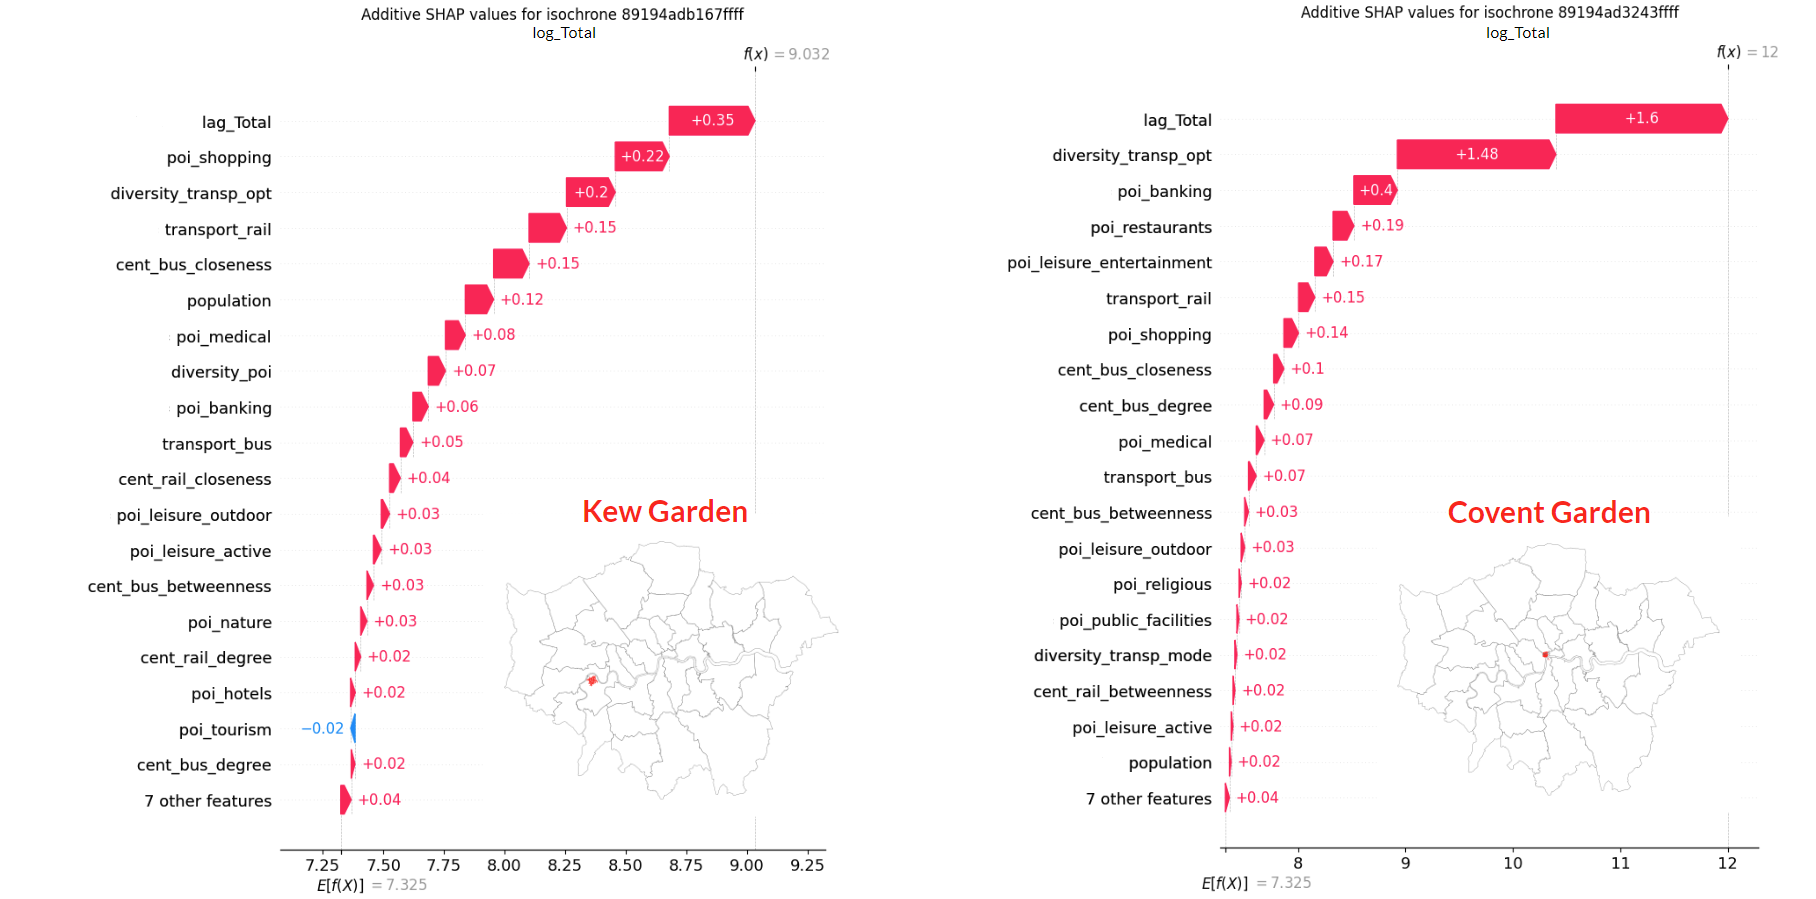
\includegraphics[width=\textwidth]{localshap.png}
    \captionsetup{justification=centering}
    \caption{Local SHAP values for 2 spatial units\\Kew Gardens and Covent Garden}
    \label{fig:localshap}
\end{figure}

By mapping the local SHAP values for all spatial units in the Greater London area, we can visualise the differing impact of the input features on the target variable across the region of interest. Figure \ref{fig:shapraw} shows the local SHAP values for two features, Outdoor leisure POIs and Entertainment leisure POIs, for the target variable of \textit{Total arrivals (log)}. The map shows that the impact of these features on the target variable is not uniform across space, with some areas showing a positive impact (red) and others showing a negative impact (blue). Central London understandably commands the highest contributions of entertainment POIs to predict trip attractiveness. Still, it also indicates secondary areas of high impact in the outer boroughs, such as Brixton and Haringey. Outdoor leisure POIs, on the other hand, have a more dispersed impact citywide, with a hotspot around Richmond. 

On the temporal dimension across time bands, we can also observe the varying impact of the input features on the target variable across different time bands. Figure \ref{fig:shapweightedtimeband} depicts local SHAP values spatial distribution throughout the day normalised by the target variable (arrival by time band) to enable comparison. Entertainment POIs in Central London have the highest trip attractiveness in Midday, especially Evening time bands. In contrast, Outdoor leisure POIs show a more consistent impact across time bands, with a notable increase in the intensity of certain hotspots and coldspots in the Late time band. 

While it is not immediately clear why this surfaces, it reveals a shortcoming in the methodology when examining the temporal effect of the feature contribution to trip attractiveness among different features. According to global feature importance for the Late time band (see Figure \ref{fig:beeswarmtimeband} in Appendix), \textit{outdoor leisure POIs} seem to have an increased impact on the prediction contrary to the expectation that no passengers would be visiting outdoor leisure POIs after midnight. Since SHAP's goal is to ultimately approximate how a trained model makes decisions, it may overestimate the importance of existing features when omitted features could have explained the variances better. This also means that the choice of the model training methodology and the feature selection process so far may not be a one-size-fits-all for temporal datasets, and additional features might be necessary to avoid overinflating the contribution of certain features for individual time bands. 

\begin{figure}[ht]
    \centering
    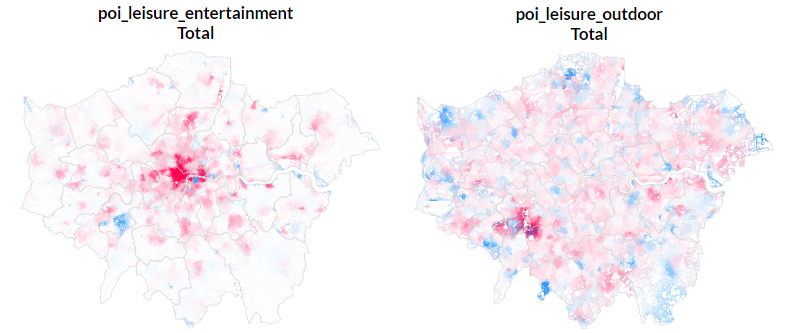
\includegraphics[width=\textwidth]{shaprawlocal.png}
    \captionsetup{justification=centering}
    \caption{Mapping local SHAP values for two features: Outdoor leisure POIs and Entertainment leisure POIs. Target: Total arrivals (log)}
    \label{fig:shapraw}
\end{figure}

\begin{figure}[ht]
    \centering
    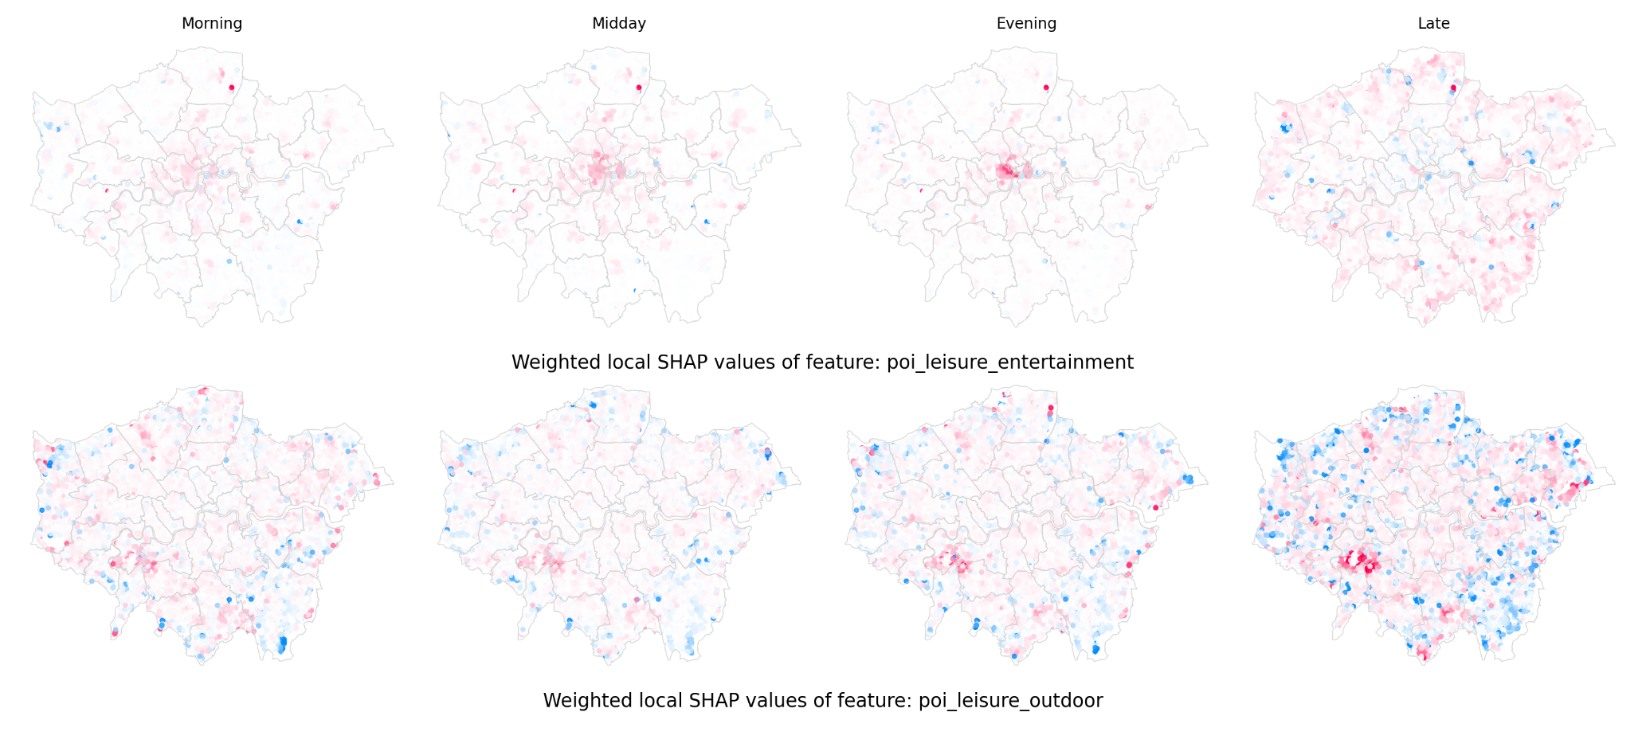
\includegraphics[width=\textwidth]{shapweightedtimeband.png}
    \captionsetup{justification=centering}
    \caption{Mapping local SHAP values for two features: Outdoor leisure POIs and Entertainment leisure POIs, weighted by number of arrivals}
    \label{fig:shapweightedtimeband}
\end{figure}

Finally, the availability of raw SHAP values also enables other manipulations for specific purposes. For example, with different types of weightage, we can observe the impact of the features on the target variable in a different light. Figure \ref{fig:shaprawweighted} shows the comparison of raw and weighted SHAP values for two features, Outdoor leisure POIs and Entertainment leisure POIs, for the target variable \textit{Total arrivals (log)}, weighted in two different ways:

\begin{enumerate}
    \setlength\itemsep{0em}
    \item Weighted by amenity diversity index: This can add more highlights to feature hotspots in areas with many other potential \textit{contenders} for trip arrivals. Under this treatment, we can see that Entertainment POIs have an even more pronounced impact in Central London and clusters of small areas with high amenity diversity, indicating that these Entertainment POIs attract trips even though the area is saturated with other amenities.
    \item Weighted by transport route option diversity index: This can add more highlights to feature hotspots in areas not well-served by many public transport routes. Under this treatment, we can see that Outdoor POIs on the outskirts of London now have a more pronounced trip attraction factor, indicating that despite the lack of public transport connectivity, these Outdoor POIs are still relatively popular.
\end{enumerate}

\begin{figure}[!hbt]
    \centering
    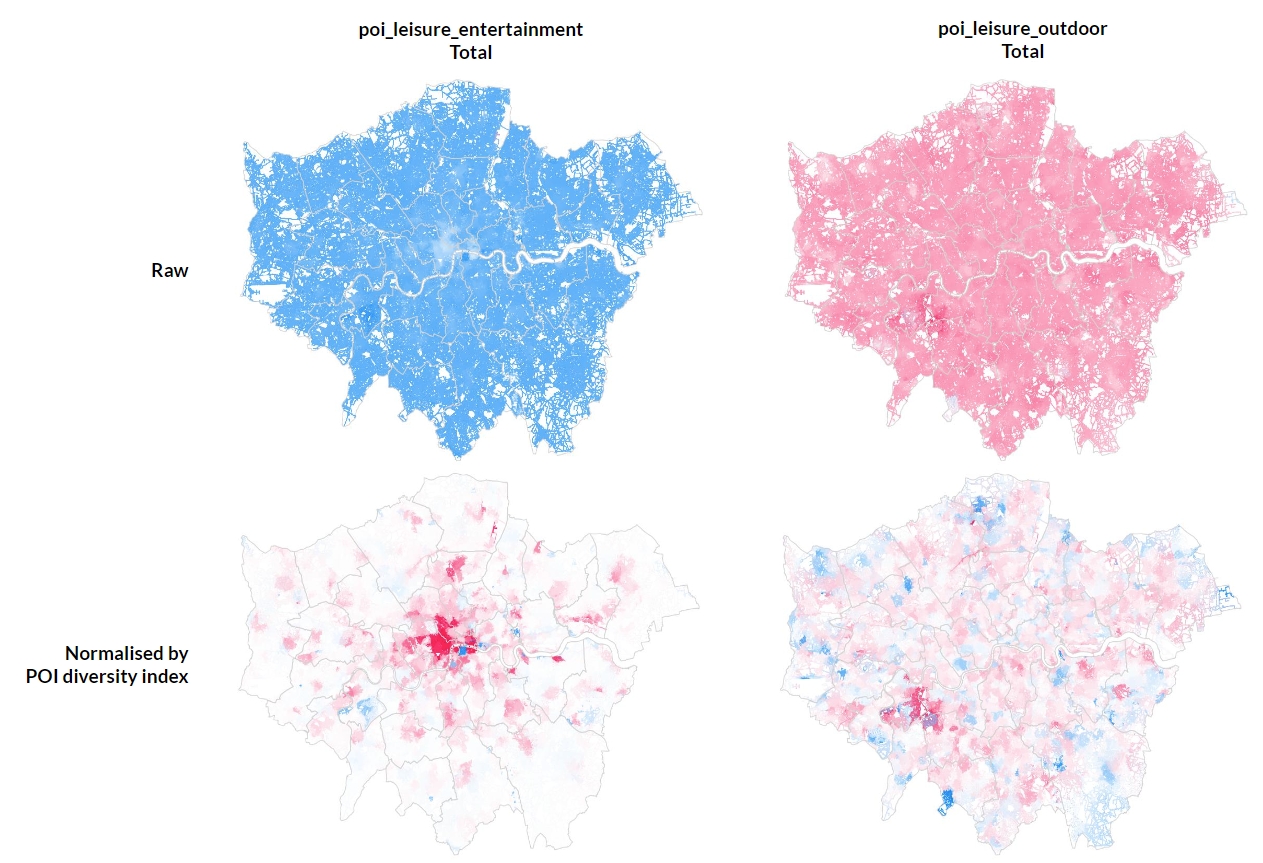
\includegraphics[width=\textwidth]{shaprawweighted.png}
    \captionsetup{justification=centering}
    \caption{Raw vs. weighted SHAP for 2 features\\Outdoor leisure POIs and Entertainment leisure POIs \\Total arrivals (log)}
    \label{fig:shaprawweighted}
\end{figure}

Overall, SHAP local interpretability with individual SHAP values for each spatial unit provides a more nuanced understanding of the impact of the input features on the target variable across space and, in our case, time. This is particularly useful for identifying activity hotspots in the Greater London area, as it allows us to pinpoint areas where certain features have a high impact on the prediction of trip attractiveness in the form of \textit{Total arrivals (log)}. Limitations exist, however, in the methodology as the comparative power of SHAP is diminished when models predicting many target variables are involved, as they are much more adept at enabling comparison of feature importance within the same model rather than across models, such as in the case of different time bands. In our discussion, we will also consider the implications and applications of these findings on urban analytics literature and transport planning.